\chapter{Convergence de Suite de Variables Aléatoires}

\justify

\setlength{\parindent}{0pt}
\renewcommand{\labelitemi}{\textbullet} % Utiliser des points noirs (•)

% ==================================================================================================================================
% Introduction 

Dans ce chapitre nous considérons un espace probabilisé $(\Omega, \mathcal{F}, \myP)$ où toutes les variables 
aléatoires sont discrètes ou à densité. 

% ==================================================================================================================================
% Suites de variables aléatoires 

\section{Suites de variables aléatoires}

\subsection{Généralités}

Commençons tout d'abord par définir formellement les suites de variables aléatoires et étudions quelques-unes 
de leurs propriétés. 

\begin{definition}[Suite de variables aléatoires]
    Soit $(\Omega, \mathcal{F}, \myP)$ un espace probabilisé. On appelle suite de variables 
    aléatoires une suite $(X_n)_{n \in \N}$ telle que :
        \[ \forall n \in \N, \quad X_n : 
            \begin{cases}
                \Omega \longrightarrow E \\ 
                \omega \longmapsto X(\omega)
            \end{cases} \text{ est une fonction mesurable} \] 
    Dans le cas où $E = \R$ on parlera de suite de variables aléatoires réelles. 
\end{definition}


\begin{definition}[Suite i.i.d.]
    Soit $(X_n)_{n \in \N}$ une suite de variables aléatoires définies sur un espace probabilisé 
    $(\Omega, \mathcal{F}, \myP)$. 
    
    \begin{itemize}
        \item On dit que la suite est \emph{identiquement distribuée} si toutes les variables $X_n$ ont la même loi :
        \[ \forall n \in \N, \quad X_n \sim \mathcal{L}. \]
        
        \item On dit que les variables sont \emph{indépendantes} si, pour tout $n \in \N$ et tout $(A_1, \dots, A_n) \in \mathcal{B}_\R$, on a :
        \[ \myP\left( \bigcap_{k = 1}^{n} \{ X_k \in A_k \} \right) = \prod_{k = 1}^{n} \myP(X_k \in A_k) \]
        (Cette condition traduit l'indépendance des variables aléatoires en termes de lois de distribution.)
    \end{itemize}
    
    Lorsque $(X_n)$ est à la fois indépendante et identiquement distribuée, on dit que c’est une suite \emph{i.i.d.}
\end{definition}

Les suites de variables aléatoires sont très utiles en modélisation. En effet elles peuvent servir à : 
\begin{itemize}
    \item La modélisation d'une expérience répétée : comme $n$ lancers d'une pièce de monnaie ou $n$ relevés de température. 
    \item Relever des séquences de mesures aléatoires : en statistiques, on collecte souvent des données issues d'un même échantillon 
    aléatoire via le processus d'échantillonnage. Cela revient à considérer une suite de variables aléatoires 
    $(X_n)_{n \in \N}$ telle que les $X_n$ sont : 
        \begin{itemize}
            \item définies sur un même espace probabilisé 
            \item souvent identiquement distribuées 
            \item et indépendantes
        \end{itemize}
\end{itemize}

\begin{example}[Simple]
    Considérons l'expérience aléatoire de $n$ lancés d'une pièce équilibrée non truquée. 
    On a alors $ \Omega = \{\text{ Pile}, \text{ Face}\} = \{p,f\}$ et soit la suite de variables 
    aléatoires $(U_n)_{n \in \N}$ définie sur $(\Omega, \mathcal{F}, \myP)$ telle que :
        \[ U_n = 
            \begin{cases}
                0 \quad \text{si le nième lancer donne Pile} \\ 
                1 \quad \text{si le nième lancer donne Face} \\ 
            \end{cases}
        \]
    Alors $(U_n)_{n \in \N}$ est une suite de variables aléatoires de Bernouilli $ \mathcal{B}(1/2)$, 
    indépendantes et identiquement distribuées. 
\end{example}


\subsection{Exemple Introductif : lancer d'une pièce}

Reprenons un exemple classique : le lancer d’une pièce de monnaie. Soit $(X_n)_{n \in \N^*}$ une suite 
de variables aléatoires modélisant les résultats successifs d’un tel lancer. On modélise l’espace probabilisé 
par l'univers : $\Omega = \{s, \overline{s}\}^{\N^*} $ où $s$ désigne un « succès » (par exemple, pile) 
et $\overline{s}$ un « échec » (face), et où chaque élément $\omega \in \Omega$ est une suite infinie de 
résultats.

On suppose que les $X_n$ sont des variables de Bernoulli de paramètre $p \in [0,1]$ :
    \[
        \forall n \in \N^*,\quad \mathbb{P}(X_n = 1) = p \quad \text{et} \quad \mathbb{P}(X_n = 0) = 1 - p.
    \]
Cela signifie que chaque lancer est indépendant des précédents, et a une probabilité $p$ de donner $1$ (succès).

\vspace{0.3cm}

Considérons la variable aléatoire suivante :
    \[
        X_n := \frac{1}{n} \sum_{k=1}^n X_k.
    \]
Elle représente la fréquence de succès (i.e. de « pile ») parmi les $n$ premiers lancers.
Intuitivement, on s’attend à ce que cette fréquence se rapproche de $p$ quand $n$ devient grand. 
C’est ce que l’on veut exprimer par une notion de convergence.

\vspace{0.3cm}

Mais si l'on regarde certaines suites particulières $\omega \in \Omega$, par exemple :
\begin{itemize}
    \item $\omega_1 = (1,1,1,1,\dots)$,
    \item $\omega_2 = (0,0,0,0,\dots)$,
    \item $\omega_3 = (0,1,1,0,1,1,0,1,1,\dots)$ (suite périodique),
\end{itemize}

on obtient :
\[
    \lim_{n \to \infty} X_n(\omega_1) = 1, \quad 
    \lim_{n \to \infty} X_n(\omega_2) = 0, \quad 
    \lim_{n \to \infty} X_n(\omega_3) = \frac{2}{3}.
\]

Ces valeurs ne sont pas égales à $p$ en général.
Autrement dit, la convergence point par point (c’est-à-dire pour chaque $\omega$ fixé) ne suffit pas à garantir que $X_n(\omega) \to p$.

\vspace{0.3cm}

Il va donc nous falloir introduire des notions de convergence plus fines, adaptées aux variables aléatoires, 
qui prennent en compte la structure probabiliste de l’espace. Cela nous amène aux différentes formes de 
convergence en probabilité. Ces outils permettent de formaliser ce que signifie réellement « $X_n$ tend 
vers $p$ » dans un contexte probabiliste.

% ==================================================================================================================================
% Convergence en probabilités

\section{Convergence en Probabilités}

\begin{definition}[Convergence en Probabilités]
    Soit $(X_n)_{n \in \N}$ une suite de variables aléatoires et $X$ une variable aléatoire sur un 
    même espace probabilisé $(\Omega, \mathcal{F}, \myP)$. On dit que la suite $(X_n)_{n \in \N}$ 
    \emph{converge en probabilité} vers la variable $X$ si : 
        \[ \forall \varepsilon > 0, \quad \lim_{n\to\infty} \myP(|X_n - X| > \varepsilon) = 0 \] 
    on note alors : $ X_n \overset{\myP}{\longrightarrow} X$. 
\end{definition}

Intuitivement, cela signifie que plus $n$ est grand, plus la probabilité que $X_n$ s'écarte significativement 
de la limite $X$ devient faible. En d'autres termes, les réalisations de $X_n$ deviennent, avec une 
probabilité croissante, arbitrairement proches de celles de $X$.

\subsection{Opérations}

\begin{prop}[Convergence en probabilités et somme]
    Soient deux suites de variables aléatoires $(X_n)_{n \in \N}$ et $(Y_n)_{n \in \N}$ telles que 
    $X_n \overset{\myP}{\longrightarrow} X$ et $ Y_n \overset{\myP}{\longrightarrow} Y$ on a alors : 
        \[ X_n + Y_n \overset{\myP}{\longrightarrow} X + Y \] 
\end{prop}

\begin{prop}[Convergence en probabilités et application continue]
    Soient une suite de variables aléatoires $(X_n)_{n \in \N}$ et $f : \R \longrightarrow \R$ une application 
    continue telles que $X_n \overset{\myP}{\longrightarrow} X$ alors, on a : 
        \[ f(X_n) \overset{\myP}{\longrightarrow} f(X) \] 
\end{prop}

\subsection{Inégalités utiles et loi faible des grands nombres}

Pour effectuer des calculs et calculer des convergences en probabilités, deux inégalités sont très utiles. 

\begin{proposition}[Inégalité de Markov]
    Soit $X$ une variable aléatoire \textbf{positive} sur un espace probabilisé $(\Omega, \mathcal{F}, \myP)$ 
    admettant une espérance, alors : 
        \[ \forall a > 0, \quad \myP (X \geqslant a) \leqslant \frac{\E(X)}{a}  \] 
\end{proposition}

\begin{proposition}[Inégalité de Bienaymé-Tchebychev]
    Soit $X$ une variable aléatoire admettant une variance, alors : 
        \[ \forall \varepsilon > 0, \quad \myP(|X - \E(X)| \geqslant \varepsilon) \leqslant \frac{V(X)}{\varepsilon^2} \] 
\end{proposition}

\begin{theorem}[Loi faible des grands nombres (version de Khinchine)]
    Soit $(X_n)_{n \in \N}$ une suite de variables aléatoires réelles, indépendantes, identiquement 
    distribuées (i.i.d), admettant une espérance $\mu = \E(X_1) < \infty$.

    Alors, la moyenne empirique :
    \[
        \bar{X}_n = \frac{1}{n} \sum_{k=1}^{n} X_k
    \]
    converge en probabilité vers $\mu$ :
    \[
        \bar{X}_n \overset{\mathbb{P}}{\longrightarrow} \mu.
    \]
\end{theorem}

Autrement dit, en répétant une même expérience aléatoire de manière indépendante, la moyenne des résultats 
observés finit par se rapprocher, avec une forte probabilité, de la moyenne théorique. 
C’est le fondement des statistiques empiriques.

\begin{corollary}[Théorème d'or de Bernouilli]
    Soit $(X_n)_{n \in \N}$ une suite de variables aléatoires de Bernouilli de même paramètre $p$. 
    Alors la moyenne empirique converge en probabilités vers $p$. 
    \[ \text{i.e} \quad \overline{X_n} = \frac{1}{n} \sum_{k=1}^{n} X_k \overset{\myP}{\longrightarrow} p \] 
\end{corollary}



C’est une version particulière de la loi faible des grands nombres appliquée à une variable de Bernoulli. 
Elle justifie l’interprétation fréquentiste des probabilités. Cela nous permet de dire que la fréquence statistique d'un évènement tend vers sa probabilité. 
Par exemple, si l’on répète un tirage « pile ou face » (avec $p = 0{,}5$) un grand nombre de fois, 
la proportion de « pile » obtenue se rapproche de $0.5$ avec une forte probabilité.


% ==================================================================================================================================
% Convergence Presque Sûre

\section{Convergence Presque Sûre}

Le modèle de convergence presque sûre s'appuie sur le fait que l'on va négliger le résultat d'évènements de 
probabilité nulle dans le calcul de la convergence. 
En effet, dans l'exemple d'introduction, nous contredisons notre hypothèse grâce à des évènnements qui sont 
en réalité presque impossible à réaliser. La probabilité qu'ils se produisent est presque nulle, on peut donc 
ne pas les considérer. C'est ce que va nous permettre la convergence presque sûre. 

\begin{definition}[Convergence presque sûre]
    Soit $(X_n)_{n \in \N}$ une suite de variables aléatoires définies sur un espace probabilisé $(\Omega, \mathcal{F}, \myP)$, et soit $X$ une variable aléatoire.
    On dit que $(X_n)$ \emph{converge presque sûrement} vers $X$ si :
    \[ \myP(\{ \omega \in \Omega, \lim_{n\to\infty} X_n(\omega) = X(\omega)\}) = 1\] 
    Autrement dit, il existe un ensemble $A \subset \Omega$ de probabilité $1$ tel que, pour tout $\omega \in A$, on ait $X_n(\omega) \to X(\omega)$.

    On note alors : \[ X_n \xrightarrow[n \to \infty]{\text{p.s.}} X \quad \text{ou} \quad X_n \overset{\text{p.s.}}{\longrightarrow} X \]
\end{definition}

Cela signifie que presque tous les scénarios de $\Omega$ (sauf un ensemble négligeable de probabilité nulle)
voient la suite $(X_n)_{n \in \N}$ tendre vers $X$. 

\begin{prop}[Comparaison]
    La convergence presque sûre est plus forte que la convergence en probabilités. 
    Soient une suite de variables aléatoires $(X_n)_{n \in \N}$ et une variable aléatoire $X$ on a alors : 
        \[ X_n \overset{p.s}{\longrightarrow} X \Longrightarrow X_n \overset{\myP}{\longrightarrow} X \] 
    La réciproque est en général fausse. 
\end{prop}


\subsection{Convergence Presque Sûre et Opérations}

\begin{prop}[Stabilité par somme et produit]
    Soient $(X_n)$ et $(Y_n)$ deux suites de variables aléatoires telles que $X_n \overset{p.s.}{\longrightarrow} X$ 
    et $Y_n \overset{p.s.}{\longrightarrow} Y$. On a alors : 
        \[ X_n + Y_n \overset{p.s.}{\longrightarrow} X + Y \quad \text{et} \quad X_n \times Y_n \overset{p.s.}{\longrightarrow} X \times Y \]
\end{prop}

\begin{prop}[Convergence presque sûre et application continue]
    Soient une suite de variables aléatoires $(X_n)_{n \in \N}$ et $f : \R \longrightarrow \R$ une application 
    continue telles que $X_n \overset{p.s.}{\longrightarrow} X$ alors, on a : 
        \[ f(X_n) \overset{p.s.}{\longrightarrow} f(X) \] 
\end{prop}


\subsection{Loi forte des grands nombres}

\begin{theorem}[Loi forte des grands nombres]
    Soit $(X_n)_{n \in \N^*}$ une suite de variables aléatoires \emph{i.i.d} d'espérance finie $ \mu = \E(X_1) $. 
    Alors la moyenne empirique converge \emph{presque sûrement} vers $\mu$ : 
        \[ \boxed{\overline{X_n} = \frac{1}{n} \sum_{k=1}^{n} X_k \underset{n \to \infty}{\overset{p.s}{\longrightarrow}} \mu} \] 
\end{theorem}

Ainsi lorsque l'on répète beaucoup de fois la même expérience aléatoire dans les mêmes conditions (hypothèse \emph{i.i.d})
la moyenne empirique des expériences successives tend vers la moyenne théorique (espérance) de façon 
quasi-certaine. 


% ==================================================================================================================================
% Convergence en Loi

\section{Convergence Loi}

En probabilités, il serait utile de pouvoir approcher asymptotiquement certaines lois par d'autres plus simples
pour simplifier les calculs mais aussi le nomre de paramètres à prendre en compte. 
Pour cela, nous devons définir un nouveau type de convergence, la convergence en loi. 

\begin{definition}[Convergence en loi]
    Soit $(X_n)_{n \in \N^*}$ une suite de variables aléatoires et $X$ une variable aléatoire. 
    On dit que \emph{$(X_n)$ converge en loi vers $X$} s’il existe convergence simple des fonctions de répartition :
    \[
        \forall x \in \R \text{ tel que } F_X \text{ est continue en } x, \quad 
        F_{X_n}(x) \xrightarrow[n \to \infty]{} F_X(x)
    \]
    où $F_{X_n}$ désigne la fonction de répartition de $X_n$, et $F_X$ celle de $X$.  

    On note alors : \( X_n \xrightarrow{\mathcal{L}} X \).

    Concrètement, cela signifie que la loi de $X_n$ devient proche de celle de $X$ lorsque $n$ devient grand.
\end{definition}

\begin{example}
    Soit $X_n \sim \mathcal{B}(n, \frac{\lambda}{n})$, alors : 
        \[ X_n \overset{ \mathcal{L}}{\longrightarrow} \mathcal{P}(\lambda) \] 
    Asymtotiquement, une loi binomiale peut être approchée par une loi de poisson, plus simple...
\end{example}

\subsection{Propriétés Fondamentales}

\begin{prop}[Lien avec la convergence en probabilités]
    Soient $(X_n)_{n \in \N^*}$ une suite de variables aléatoires et $X$ une variable aléatoire. 
    On a alors : 
        \[ \text{si } X_n \overset{\myP}{\longrightarrow} \text{ alors } X_n \overset{ \mathcal{L}}{\longrightarrow} X \] 
        La convergence en probabilités implique la convergence en loi. La réciproque est fausse en général. 
\end{prop}

\begin{prop}[Stabilité]
    Soient $(X_n)_{n \in \N^*}$ une suite de variables aléatoires, $X$ une variable aléatoire toutes deux à valeurs 
    dans $E$ et $f : E \longrightarrow F$ une fonction continue. 
    Alors : 
        \[  X_n \overset{ \mathcal{L}}{\longrightarrow} X \; \Longrightarrow \; f(X_n) \overset{ \mathcal{L}}{\longrightarrow} f(X) \] 
    La convergence en loi est donc stable par fonction continue. 
\end{prop}

% ==================================================================================================================================
% Tableau Récapitulatif

\section{Tableau Récapitulatif}

\begin{remark}[Hiérarchie des convergences]
    On a les implications suivantes entre les modes de convergence :
    \[
        X_n \xrightarrow[\text{p.s.}]{} X \quad \Longrightarrow \quad X_n \xrightarrow[\mathbb{P}]{} X \quad \Longrightarrow \quad X_n \xrightarrow[\mathcal{L}]{} X
    \]
    Les réciproques sont en général fausses.
\end{remark}


% ==================================================================================================================================
% Théorème Central Limite

\newpage
\section{Théorème Central Limite}

\subsection{Exemple Introductif}

Pour introduire le Théorème Central Limite, penchons nous tout d'abord sur un exemple simple : le lancer d'une pièce de monnaie. 
Considérons le lancer d'une pièce de monnaie équilibrée. Nous avons deux issues possibles : Pile ou Face 
de probabilité $1/2$ chacune. Effectuons plusieurs lancers successifs et calculons la probabilité 
de la somme de chaque série de lancer possible. 

\vspace{0.3cm}

Si nous effectuons un seul lancer, nous avons seulement deux possibilités : 

\begin{center}
    \begin{minipage}{0.45\textwidth}
        \centering
        \captionof{table}{Résultat d'un seul tirage}
        \begin{tabular}{c|c}
            \textbf{Résultat Tirage} & \textbf{Somme} \\
            \hline 
            0 & 0 \\ 
            1 & 1 \\ 
        \end{tabular}
    \end{minipage}
    \hfill
    \begin{minipage}{0.45\textwidth}
        \centering
        \captionof{table}{Fréquences pour un tirage}
        \begin{tabular}{c|c}
            \textbf{Somme} & \textbf{Fréquence} \\
            \hline 
            0 & 0.5 \\ 
            1 & 0.5 \\ 
        \end{tabular}
    \end{minipage}
\end{center}

En effectuant deux lancers, nous avons maintenant 4 issues possibles de l'expérience aléatoire : 

\begin{center}
    \begin{tabular}{c|c|c}
        \textbf{Résultat Tirage n°1} & \textbf{Résultat Tirage n°1} & \textbf{Somme} \\
        \hline 
        0 & 0 & 0 \\
        0 & 1 & 1 \\  
        1 & 0 & 1 \\
        1 & 1 & 2 \\ 
    \end{tabular}
    \captionof{table}{Résultat de deux tirages}
\end{center}

\begin{center}
    \begin{tabular}{c|c|c}
        \textbf{Valeur de la somme} & \textbf{Fréquence d'apparition} & \textbf{Fréquence} \\
        \hline 
        0 & 1 & $1/4 = 0.25$ \\ 
        1 & 2 & $1/2 = 0.5$ \\ 
        2 & 1 & $1/4 = 0.25$ \\ 
    \end{tabular}
    \captionof{table}{Fréquences pour deux tirages}
\end{center}

Et ainsi de suite jusqu'à 4 lancers successifs, on obtient les sommes suivantes : 

\begin{center}
    \begin{tabular}{c|c|c}
        \textbf{Valeur de la somme} & \textbf{Fréquence d'apparition} & \textbf{Fréquence} \\
        \hline 
        0 & 1 & 0.125 \\ 
        1 & 3 & 0.375 \\ 
        2 & 3 & 0.375 \\ 
        3 & 1 & 0.125 \\ 
    \end{tabular}
    \captionof{table}{Fréquences pour 4 tirages}
\end{center}

On peut donc remarquer que, graphiquement, plus le nombre de lancers successifs augmente, plus la courbe 
de fréquence se rapproche d'une courbe en cloche : la densité de la loi normale. 

\begin{figure}[h]
    \centering
    \begin{subfigure}[b]{0.45\textwidth}
        \centering
        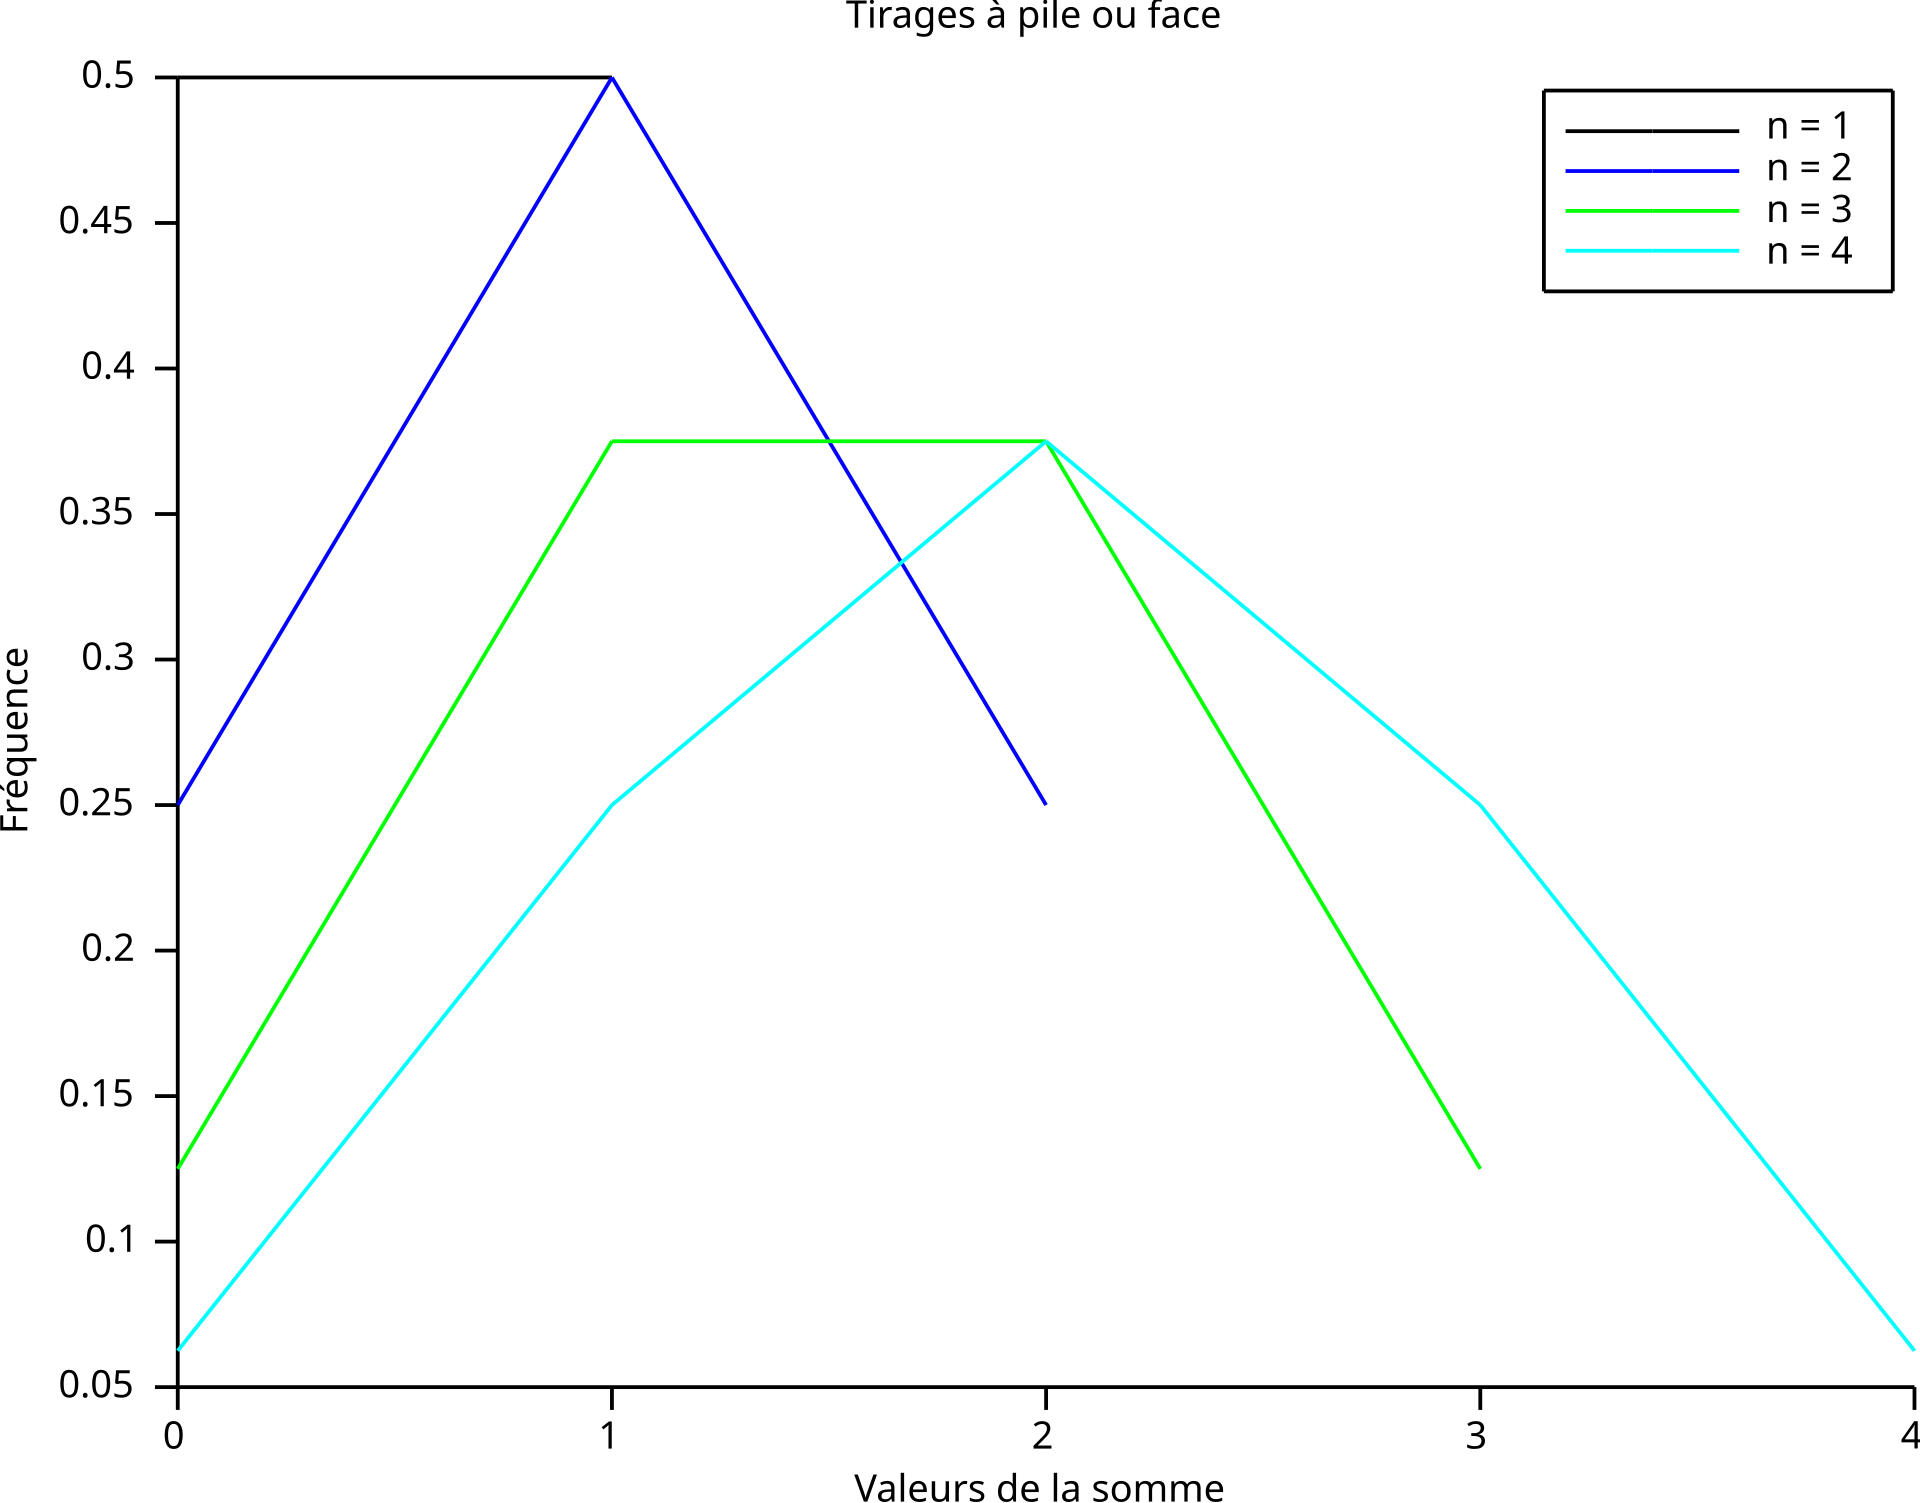
\includegraphics[width=0.7\textwidth]{images/courbe_tirages.png}
        \caption{Fréquence d'apparition d'une valeur pour la somme de $1 \leqslant n \leqslant 4$ tirages}
    \end{subfigure}
    \hfill
    \begin{subfigure}[b]{0.45\textwidth}
        \centering
        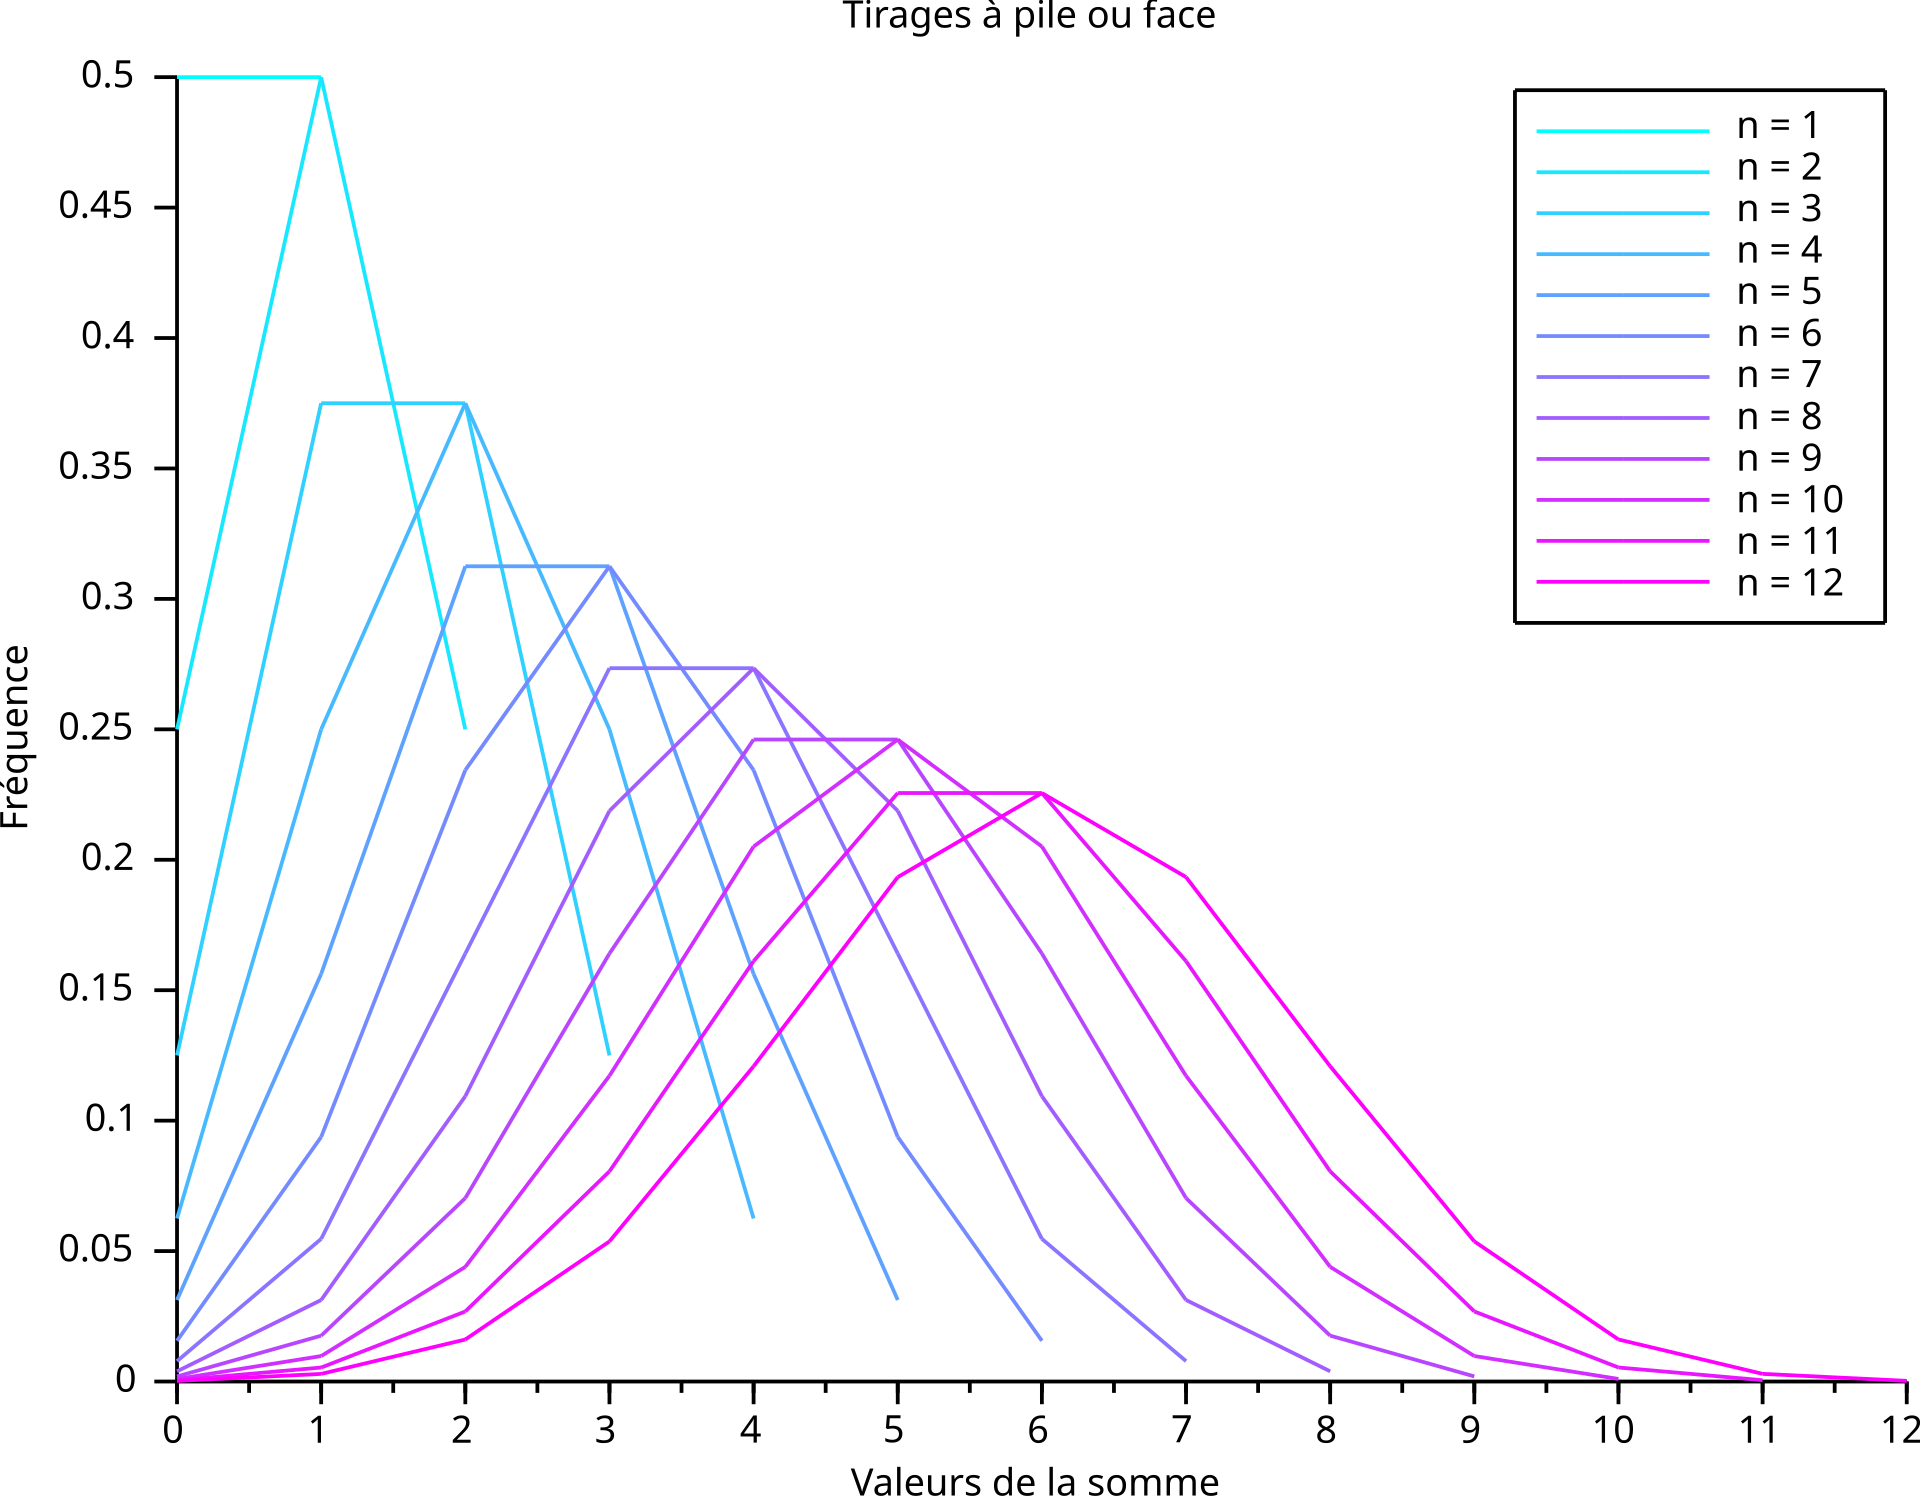
\includegraphics[width=0.7\textwidth]{images/courbe_tirages_12.png}
        \caption{\emph{Idem} pour $1 \leqslant n \leqslant 12$ tirages}
    \end{subfigure}
    \caption{Évolution de la fréquence d'apparition des sommes selon le nombre de tirages}
\end{figure}

Et cela pour n'importe quelle suite d'expériences aléatoires \emph{i.i.d}, la fréquence des sommes des issues obtenues 
"tend" vers la loi normale graphiquement. On peut interpréter de façon plus intuitive cette distribution. 
En effet, on peut se dire qu'il existe plus de façon d'effectuer un lancer qui se rapproche de la moyenne (centre de la courbe)
plutôt qu'un lancer improbable (aux extrémitées de la courbe). D'où cette distribution en cloche. 

\subsection{Théorème Central Limite}

Formalisons et généralisons ce que nous venons de voir avec un exemple. 

\begin{theorem}[Central Limite]
    Soit $(X_n)_{n \in \N^*}$ une suite de variables aléatoires \emph{i.i.d} admettant une moyenne et 
    une espérance telles que : 
        \[ \mu = \E(X_1) \quad \sigma^2 = \V(X_1) \] 
    Posons $S_n$ la somme des $n$ premières variables de la suite et $Y_n$ la variable centrée réduite de cette somme : 
        \[ S_n = X_1 + \dots X_n \quad \text{et} \quad Y_n = \frac{S_n - n \mu}{\sigma \sqrt{n}} \]
    Alors la suite $(Y_n)$ converge en loi vers la variables aléatoire de loi $ \mathcal{N}(0,1)$ 
    (la loi normale centrée réduite) :
        \[ \text{i.e } \quad \forall x \in \R, \quad \myP(Y_n \leqslant x) \underset{n \to \infty}{\longrightarrow} \frac{1}{\sqrt{2 \pi}} \int_{- \infty}^{x} e^{-u^2/2} \; du \] 
\end{theorem}

